\subsection{Cook's membrane problem}

The Cook's membrane problem \cite{simo1990} is used herein for stability analysis of pressure. The geometry of this problem is shown in Figure \ref{fg:cook_illsutration}, in which the left hand side is fixed and the right hand side subjects a concentrated force $P=6.25$ in the $y$-direction. The material parameters are Young's modulus $E=70.0$ and Poisson's ratio $\nu=0.5-10^{-8}$.

\begin{figure}[H]
\centering
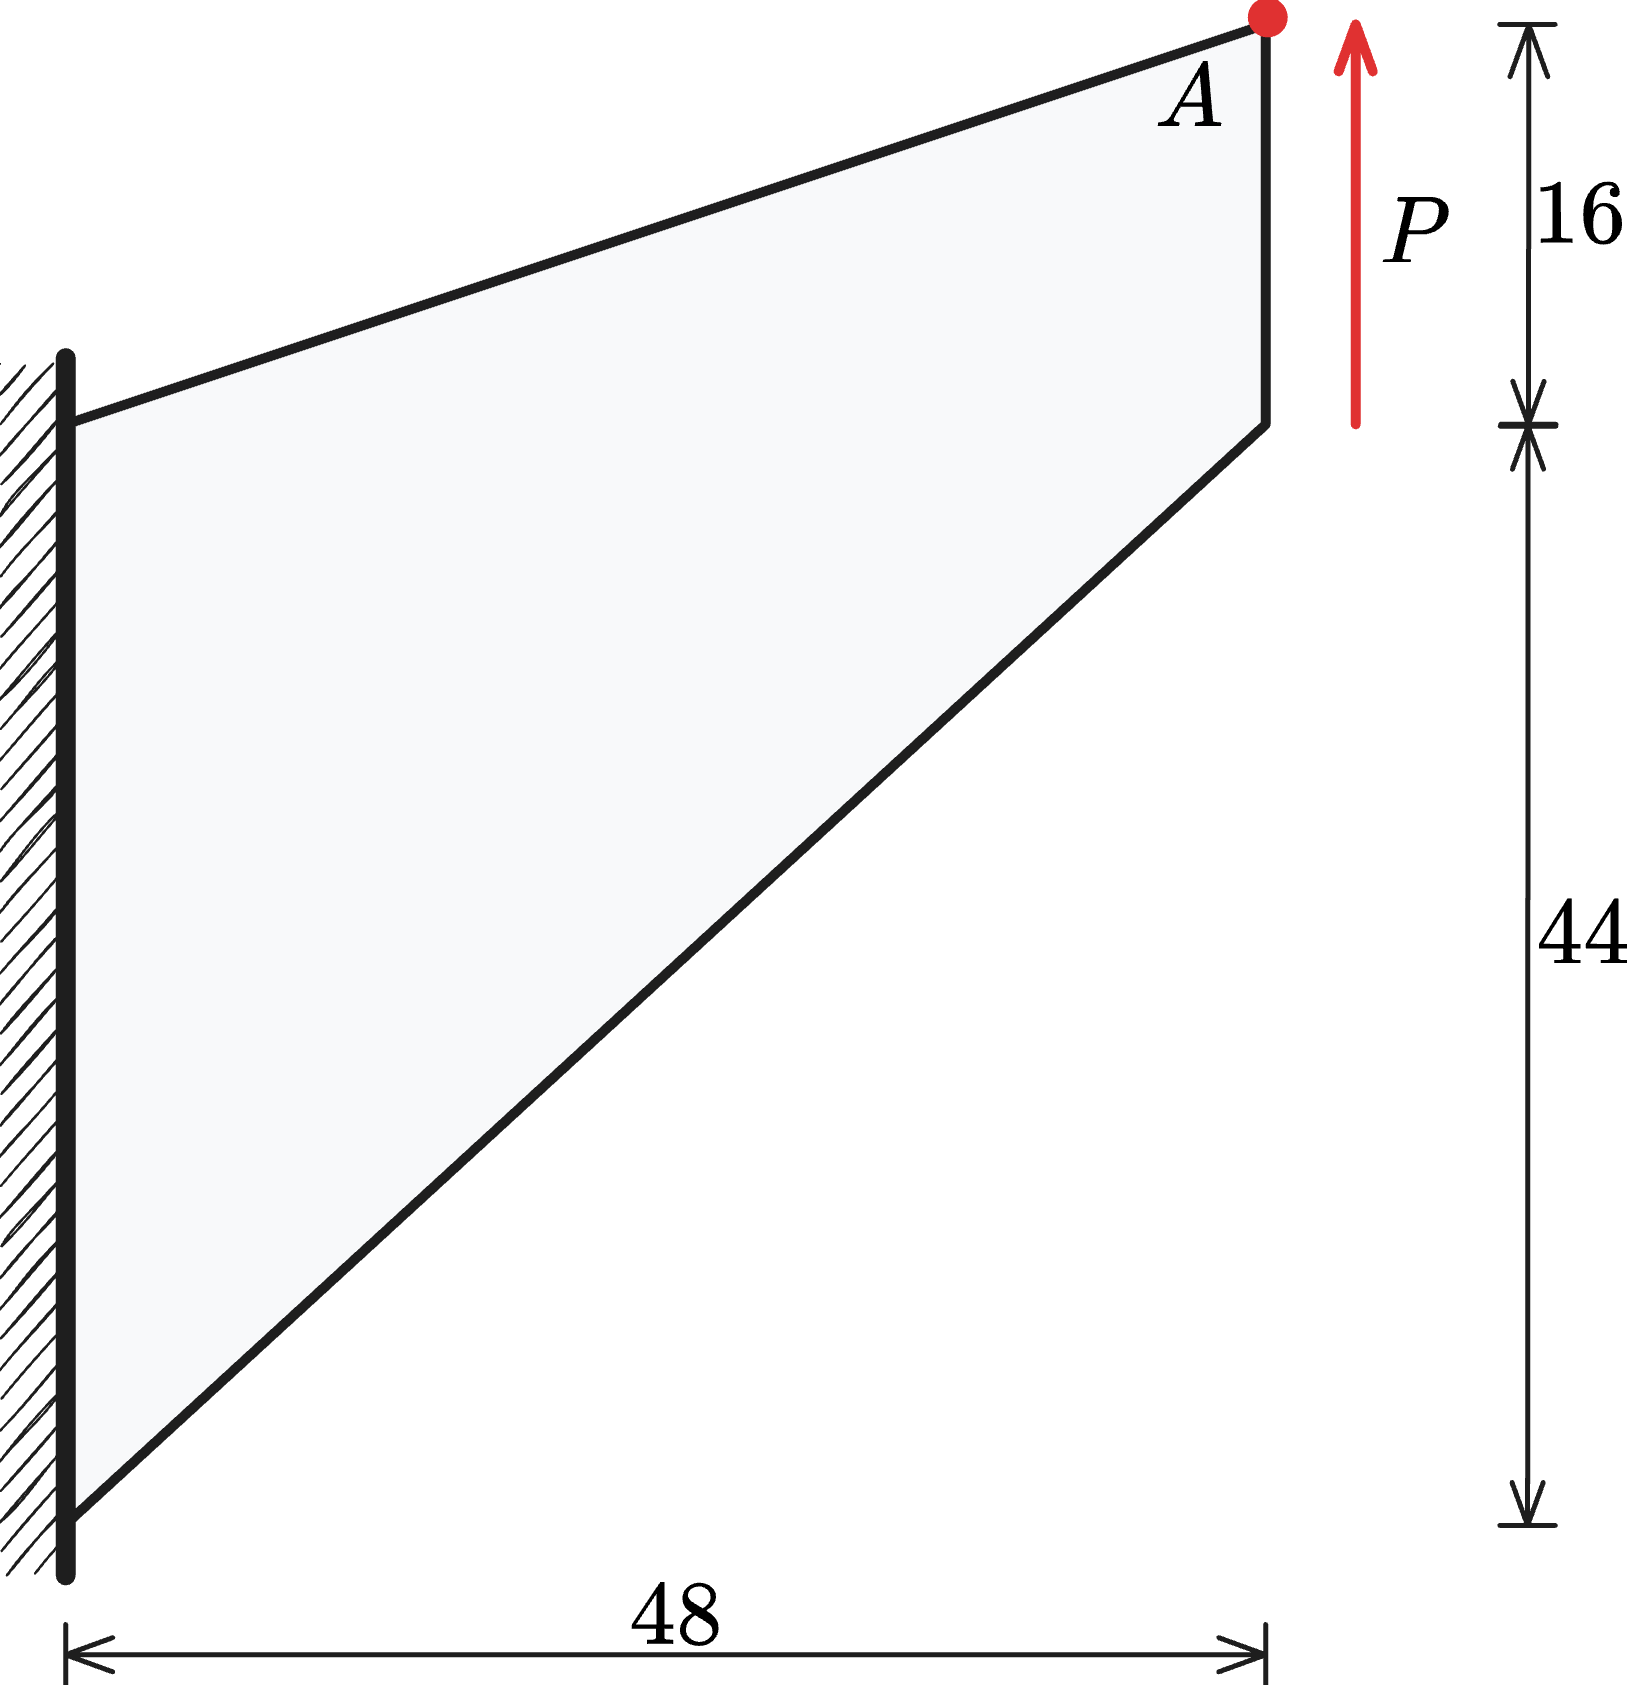
\includegraphics[width=0.5\textwidth]{png/cook_membrane_model_r1.png}
\caption{Illustration of Cook's membrane problem}\label{fg:cook_illsutration}
\end{figure}

In this test, we evaluated the convergence properties by comparing the vertical displacement at point $A$ against a reference value of $28.0$. 
As shown in Figure \ref{fg:cook_convergence} illustrates, the methods employing $r=r_{opt}$ produced results that were notably closer to this reference value than those using $r=n_d$.
Furthermore, to investigate stability, Figures \ref{fg:cook_membrane_contour_tri3}--\ref{fg:cook_membrane_contour_quad8} show the pressure contour plots for non-uniform Tri3--RK, Tri6--RK, Quad4--RK, and Quad8--RK formulations with $r=n_d$ and $r=r_{opt}$, respectively.
The reproducing kernel meshfree approximations are employed for pressure discretization with characterized support sizes of 1.5 for the linear basis function and 2.5 for the quadratic basis function. The results imply that the pressure contour plots with the optimal constraint ratio $r=r_{opt}$ show a more stable and smooth pressure distribution compared to those with the traditional constraint ratio $r=n_d$.

 \DIFaddbegin \begin{figure}[!htp]
\DIFaddendFL \centering
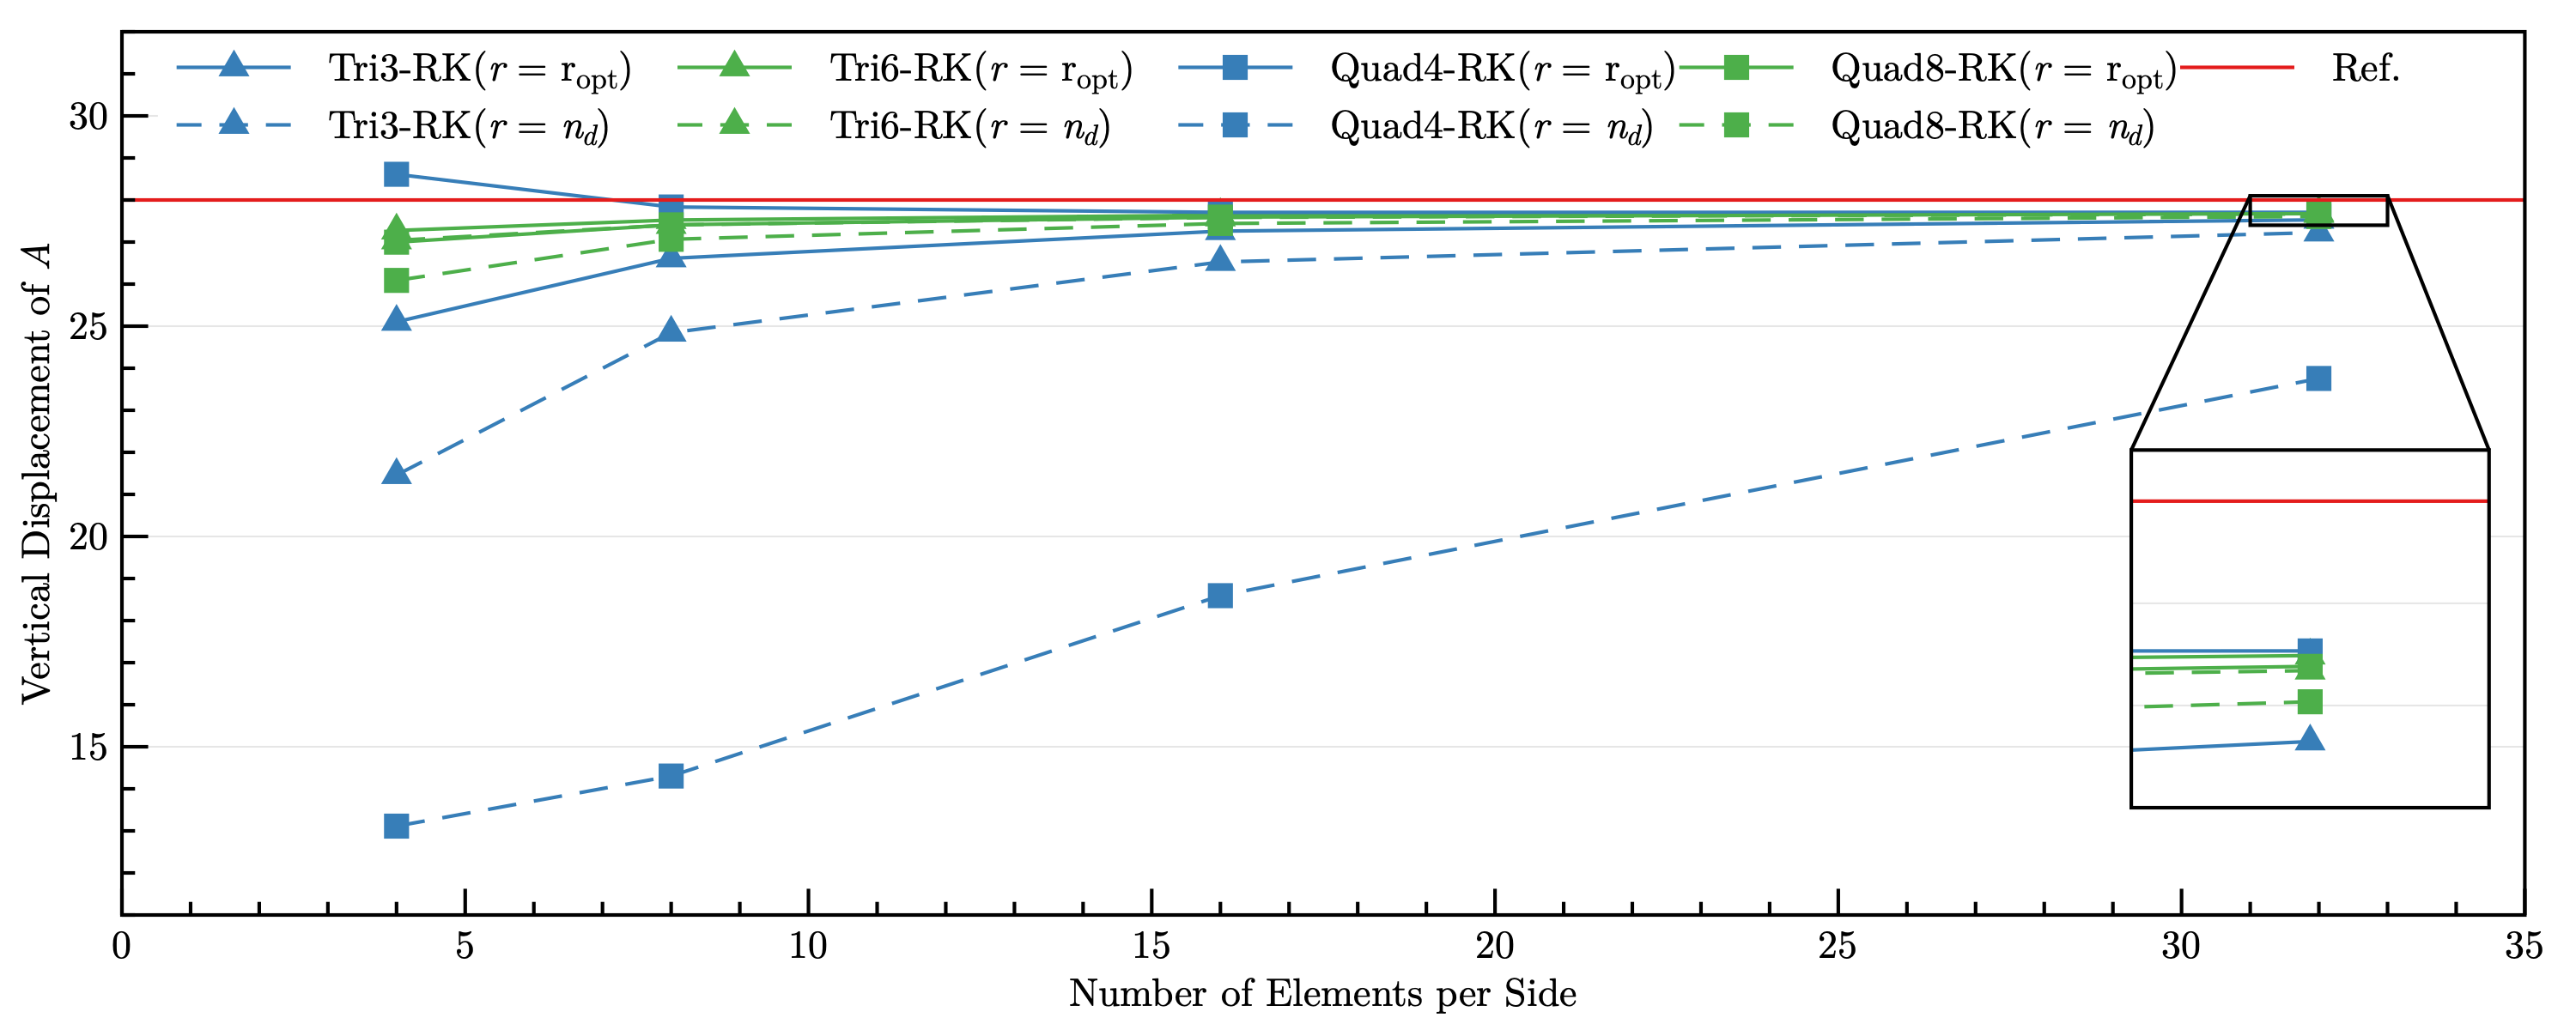
\includegraphics[width=\textwidth]{png/cook_convergence.png}
\caption{Convergence comparison of the vertical displacement at point $A$ for Cook's membrane problem}\label{fg:cook_convergence}
\end{figure}

 \DIFaddbegin \begin{figure}[!htp]
\DIFaddendFL \centering
\begin{tabular}{c@{\hspace{5pt}}c@{\hspace{5pt}}c@{\hspace{5pt}}c}
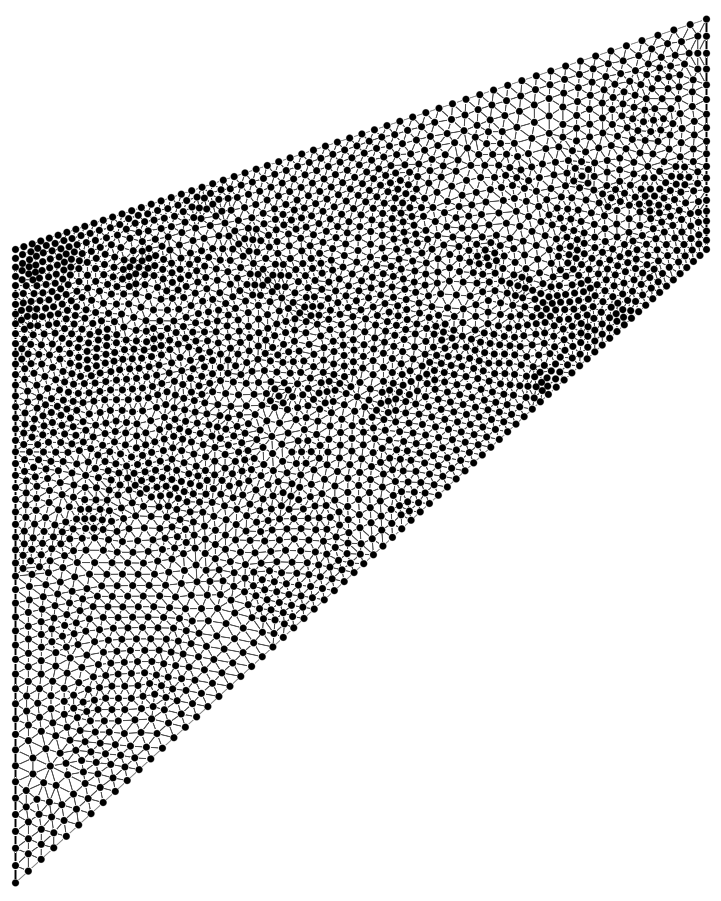
\includegraphics[width=0.33\textwidth]{png/cook_tri3_2529_msh.png}
& 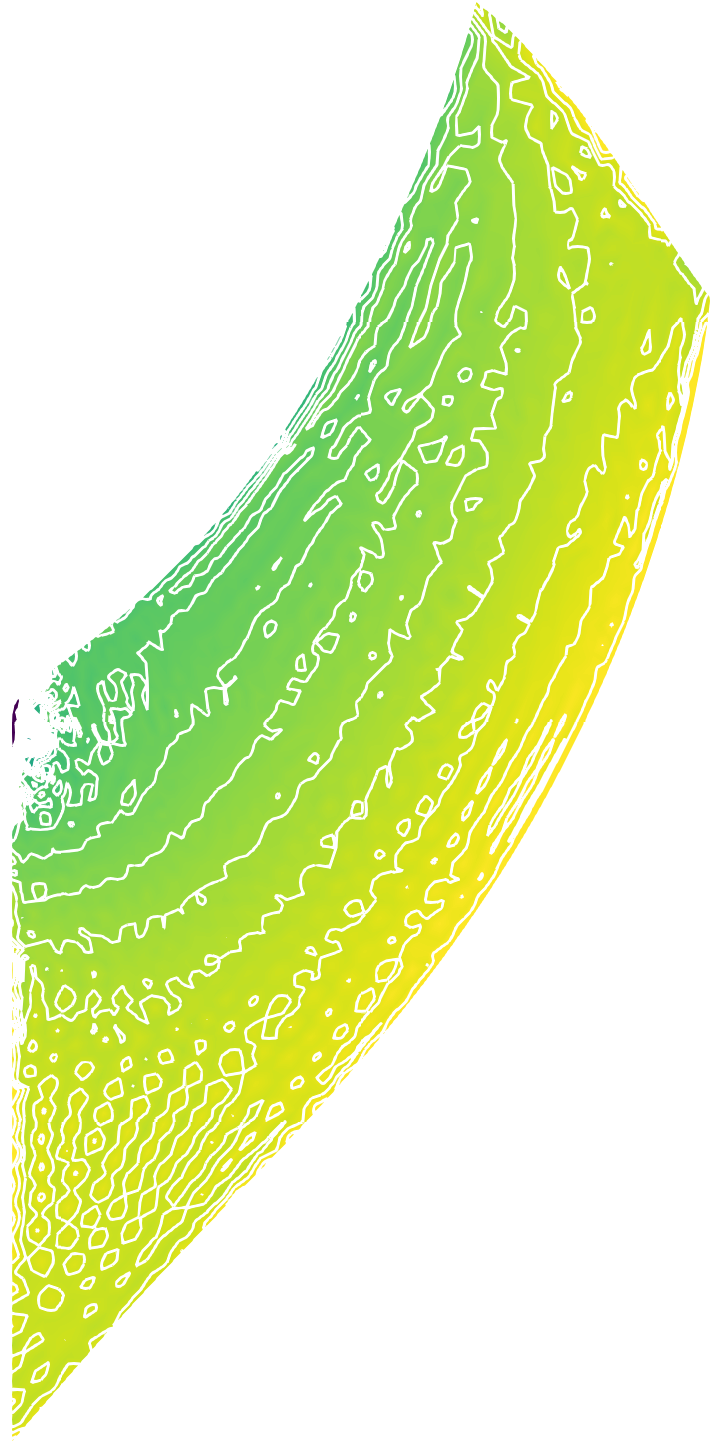
\includegraphics[width=0.28\textwidth]{png/cook_tri3_2529_2529.png}
& 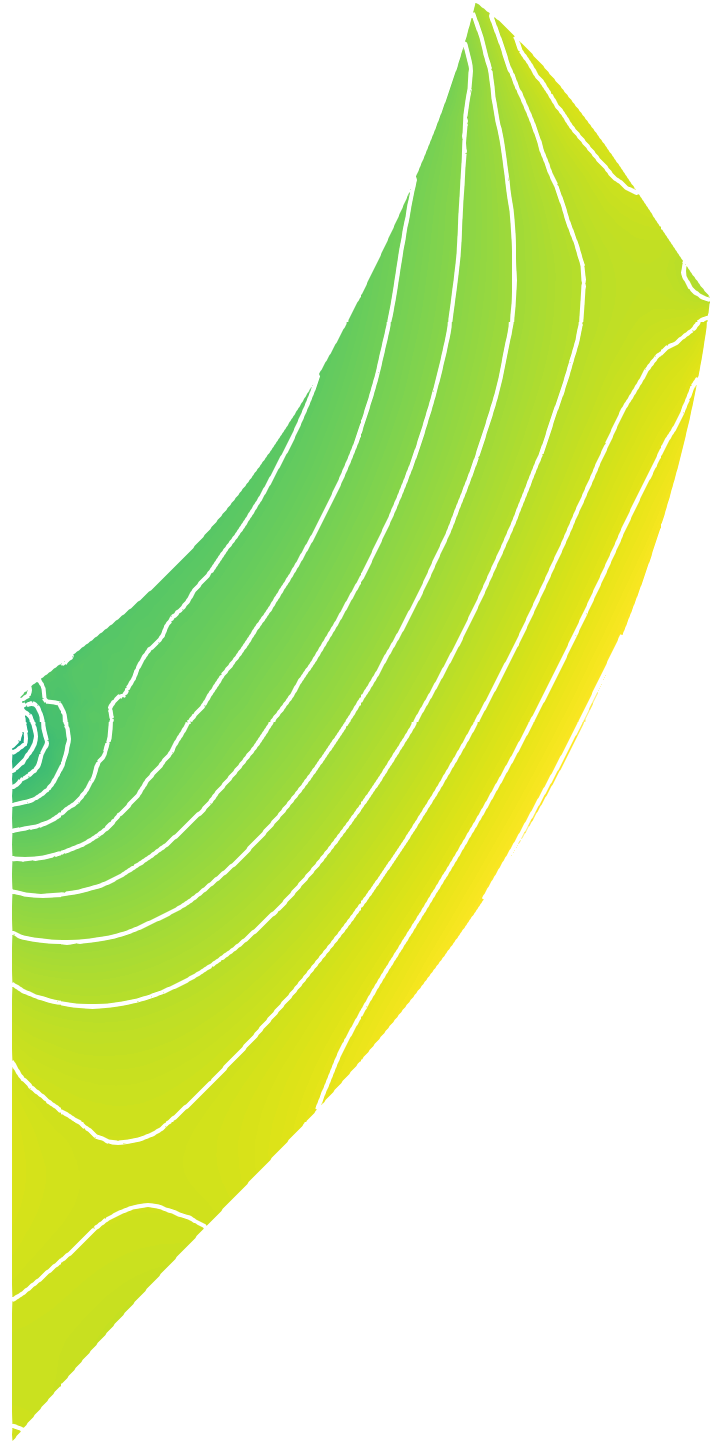
\includegraphics[width=0.28\textwidth]{png/cook_tri3_2529_658.png}
& 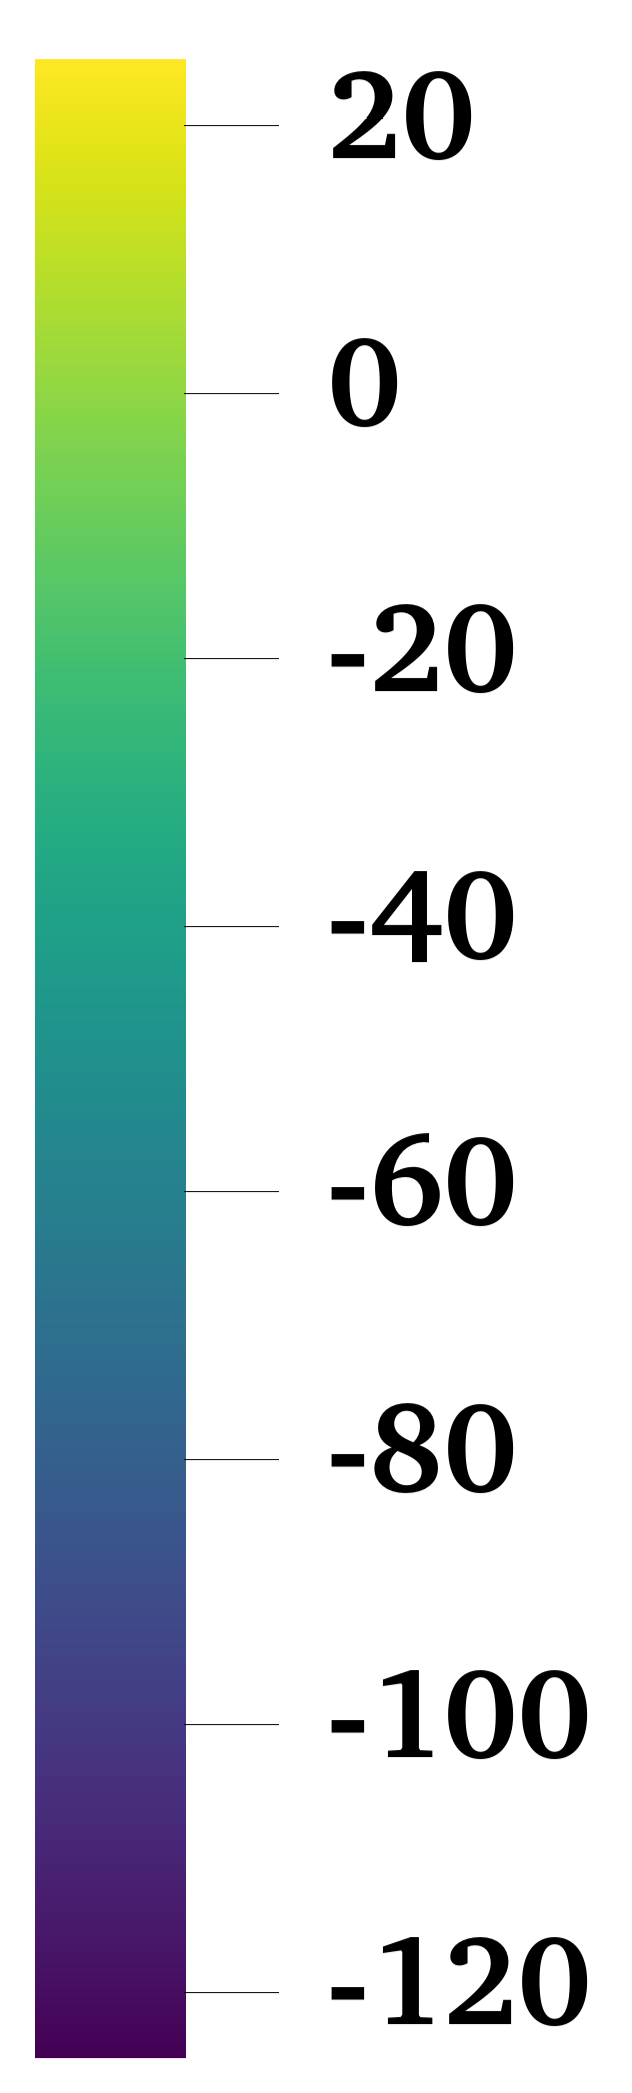
\includegraphics[width=0.1\textwidth]{png/legend.png} \\
$n_u = 2529$ & $r = n_d$ & $r = r_{opt}$ &
\end{tabular}
\caption{Pressure contour plots for Cook's membrane problem using Tri3--RK}\label{fg:cook_membrane_contour_tri3}
\end{figure}

 \DIFaddbegin \begin{figure}[!htp]
\DIFaddendFL \centering
\begin{tabular}{c@{\hspace{5pt}}c@{\hspace{5pt}}c@{\hspace{5pt}}c}
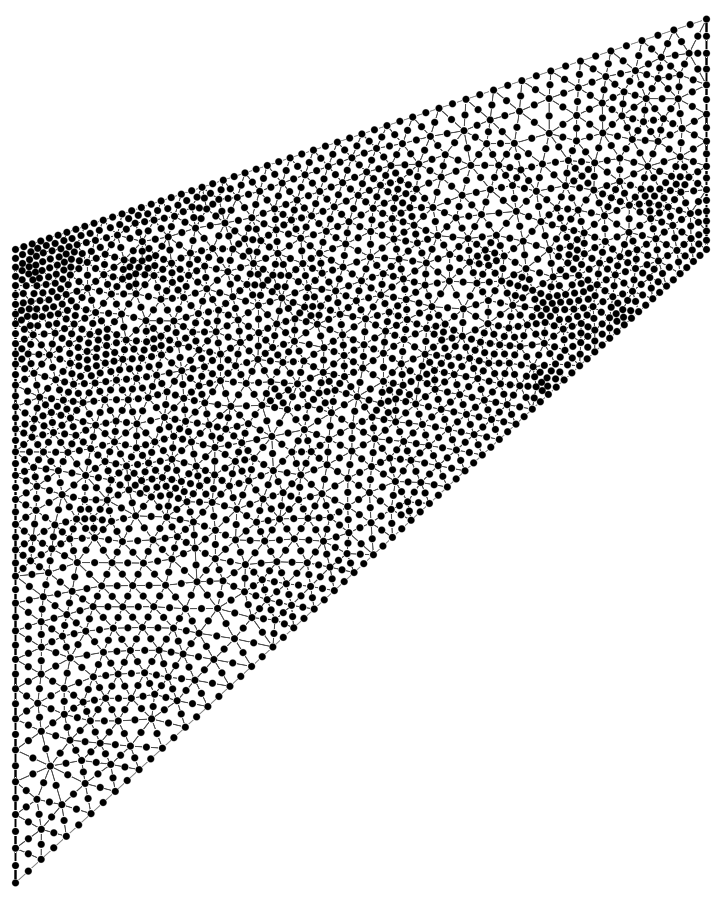
\includegraphics[width=0.33\textwidth]{png/cook_tri6_2529_msh.png}
& 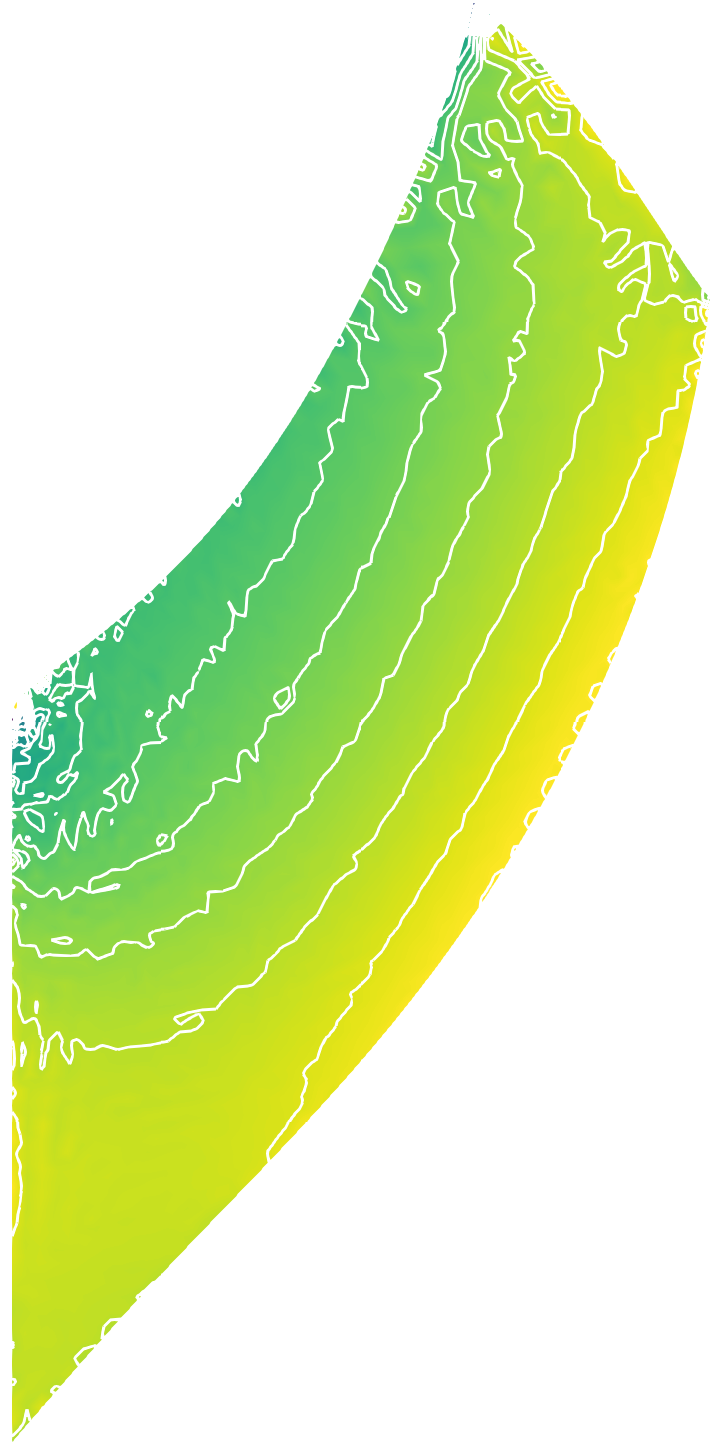
\includegraphics[width=0.28\textwidth]{png/cook_tri6_2529_2529.png}
& 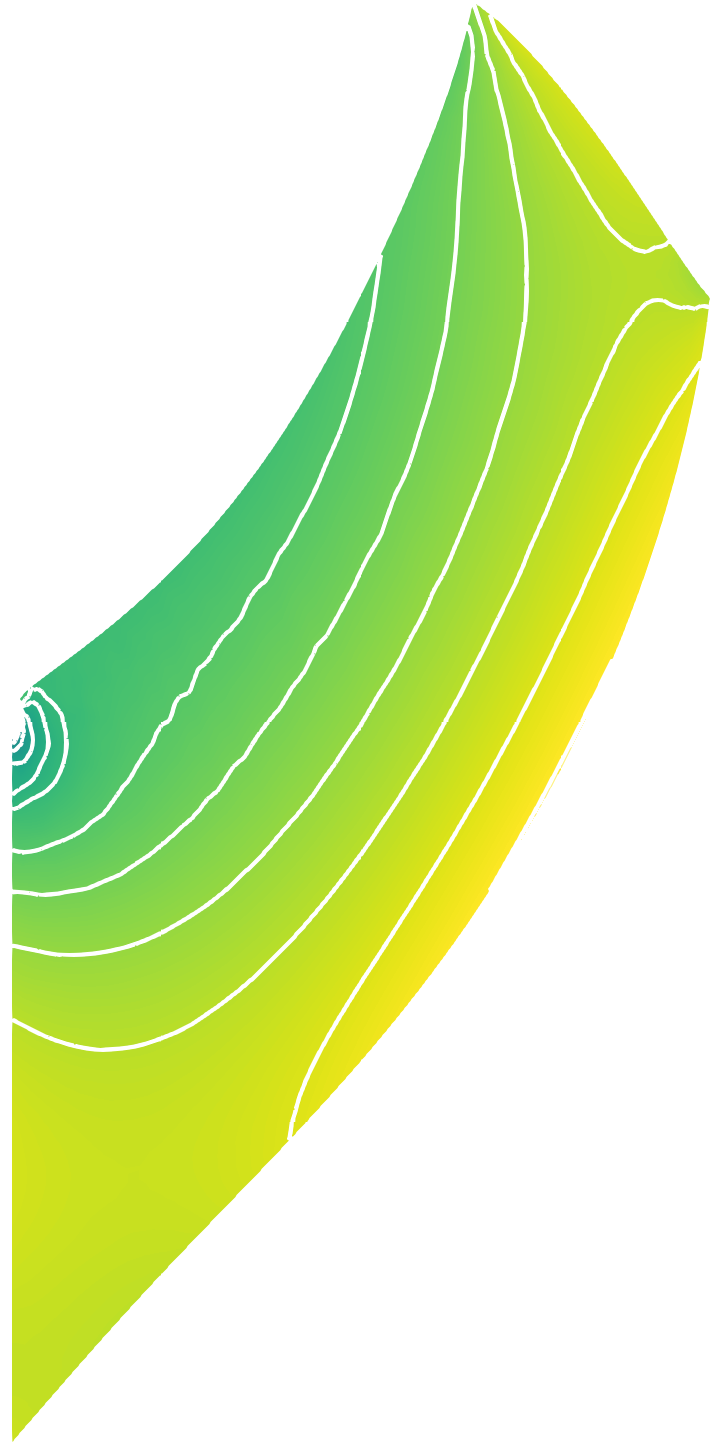
\includegraphics[width=0.28\textwidth]{png/cook_tri6_2529_658.png}
& 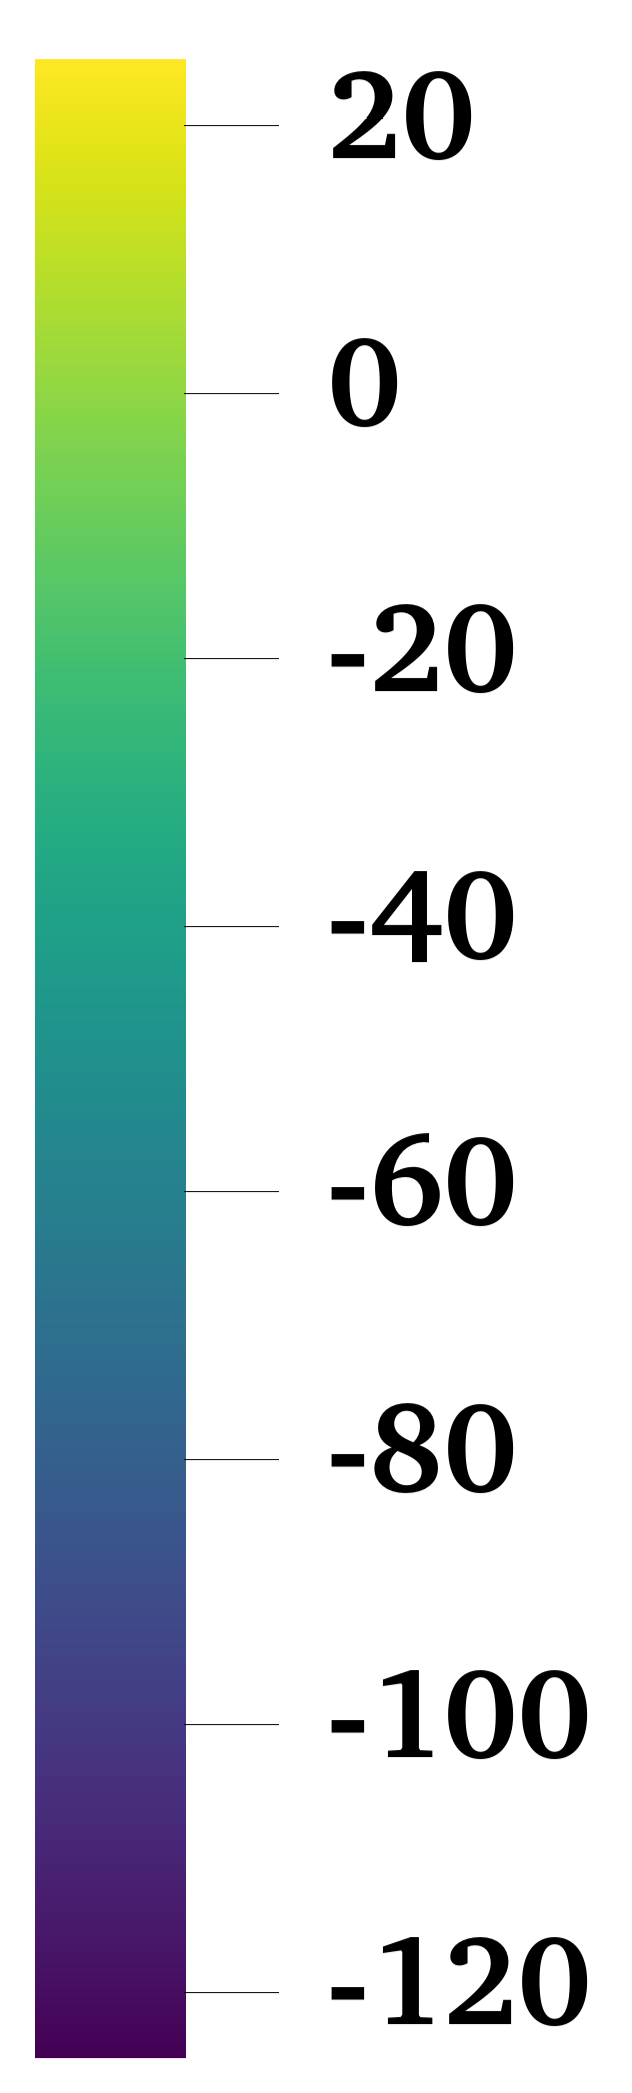
\includegraphics[width=0.1\textwidth]{png/legend.png} \\
$n_u = 2529$ & $r = n_d$ & $r = r_{opt}$ &
\end{tabular}
\caption{Comparison of pressure contour plots for Cook's membrane problem using Tri6--RK}\label{fg:cook_membrane_contour_tri6}
\end{figure}

 \DIFaddbegin \begin{figure}[!htp]
\DIFaddendFL \centering
\begin{tabular}{c@{\hspace{5pt}}c@{\hspace{5pt}}c@{\hspace{5pt}}c}
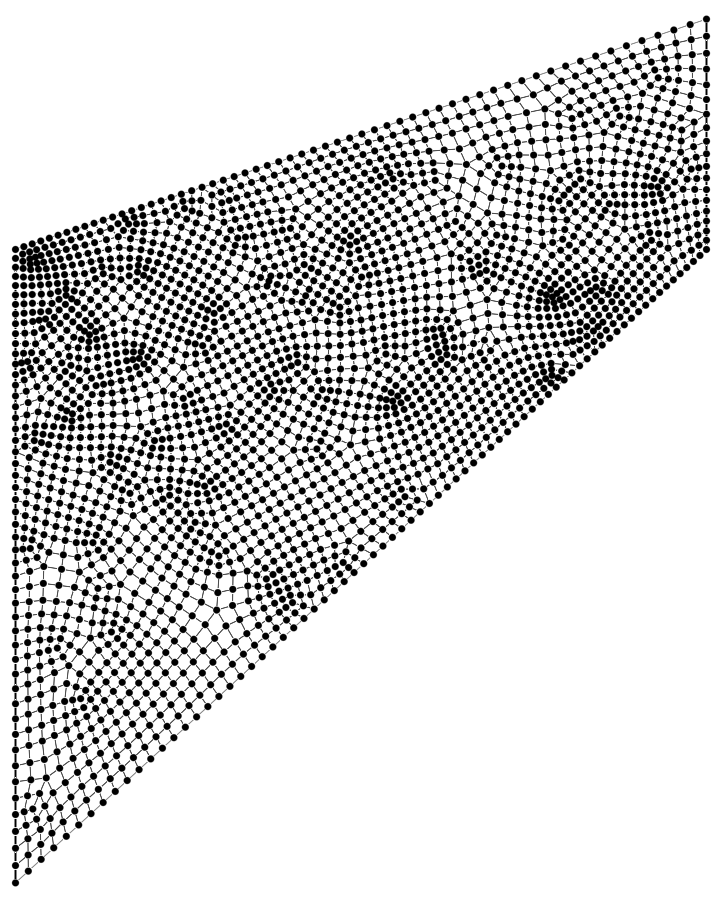
\includegraphics[width=0.33\textwidth]{png/cook_quad_2485_msh.png}
& 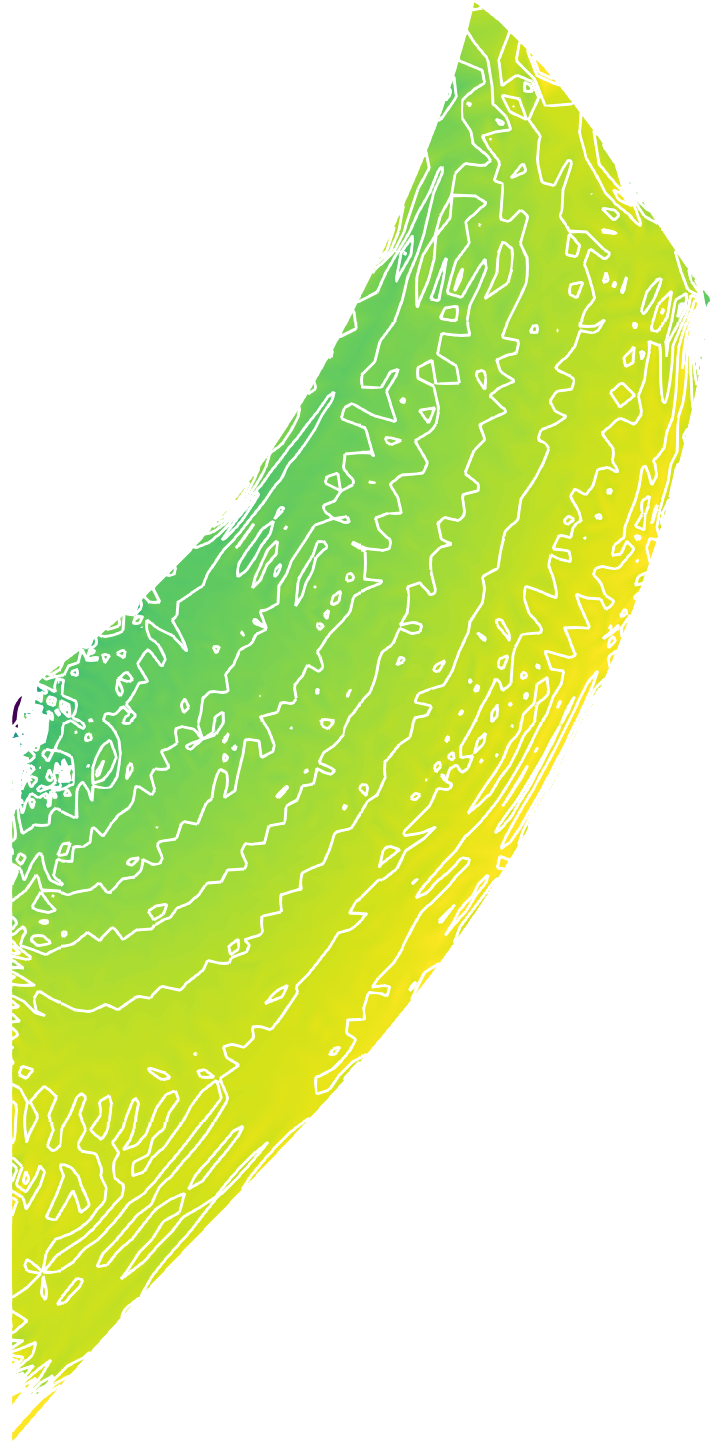
\includegraphics[width=0.28\textwidth]{png/cook_quad4_2485_2485.png}
& 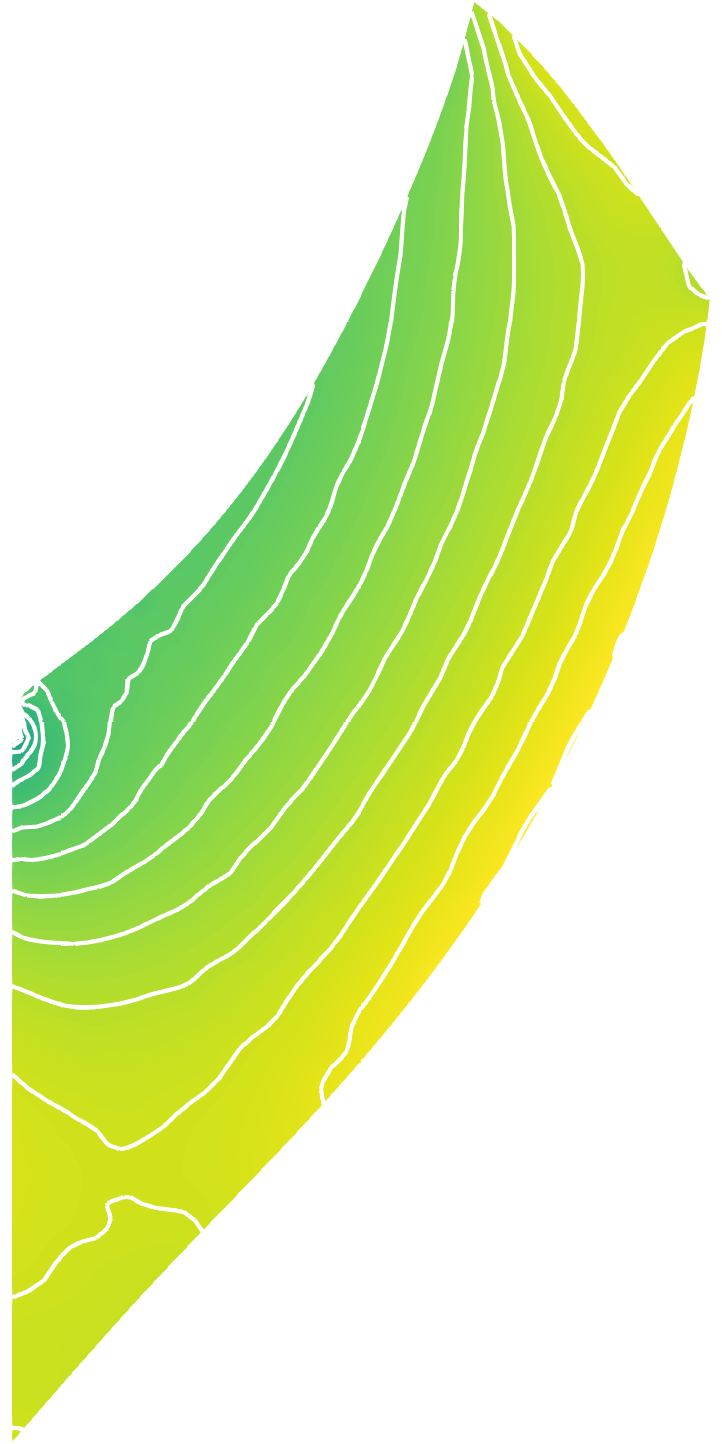
\includegraphics[width=0.28\textwidth]{png/cook_quad4_2485_647.png}
& 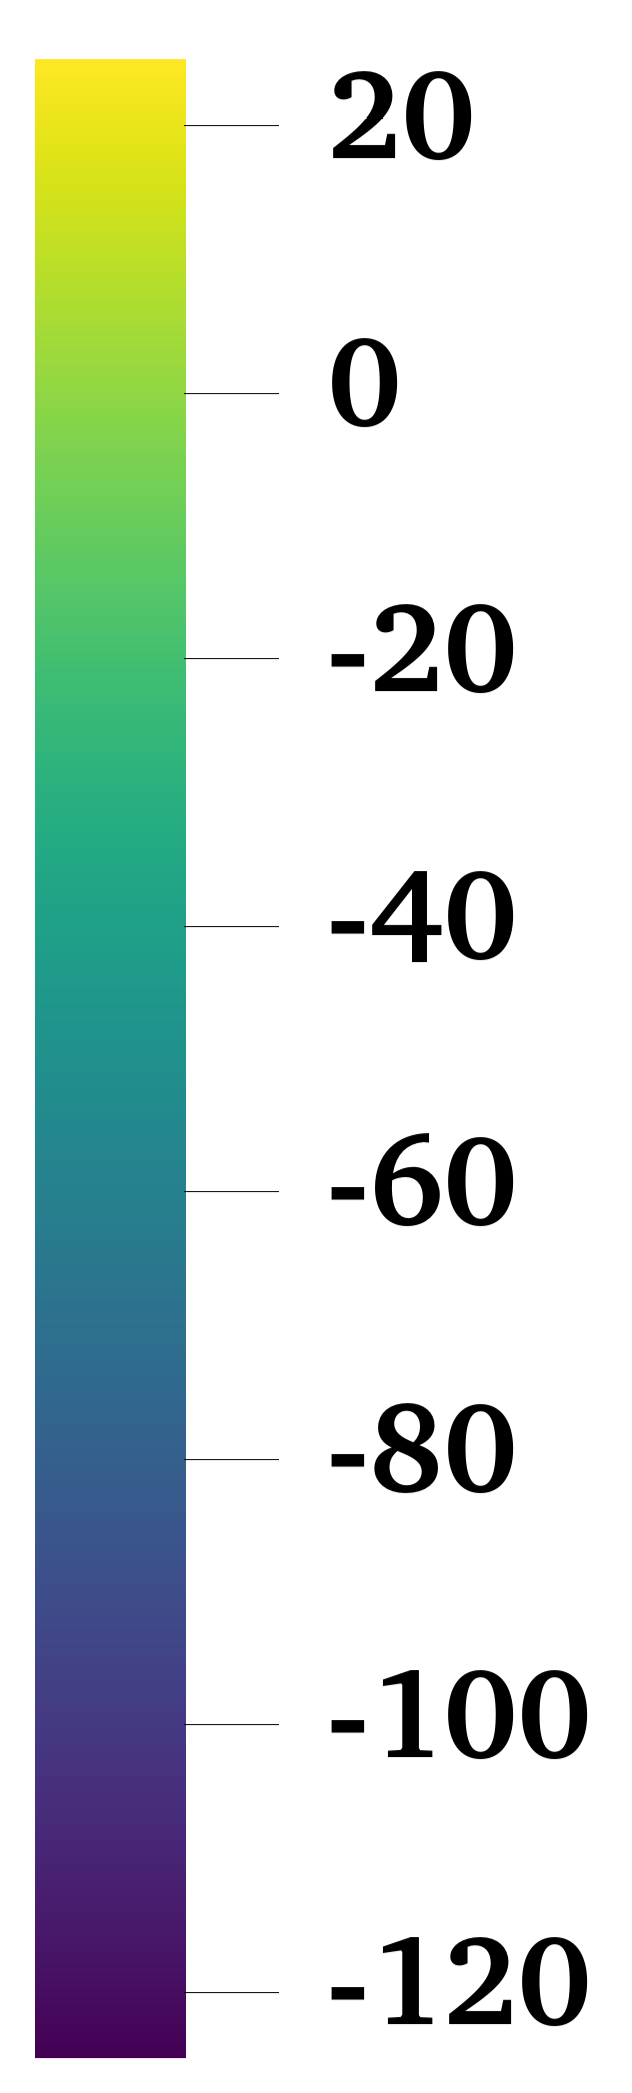
\includegraphics[width=0.1\textwidth]{png/legend.png} \\
$n_u = 2485$ & $r = n_d$ & $r = r_{opt}$ &
\end{tabular}
\caption{Comparison of pressure contour plots for Cook's membrane problem using Quad4--RK}\label{fg:cook_membrane_contour_quad4}
\end{figure}

 \DIFaddbegin \begin{figure}[!htp]
\DIFaddendFL \centering
\begin{tabular}{c@{\hspace{5pt}}c@{\hspace{5pt}}c@{\hspace{5pt}}c}
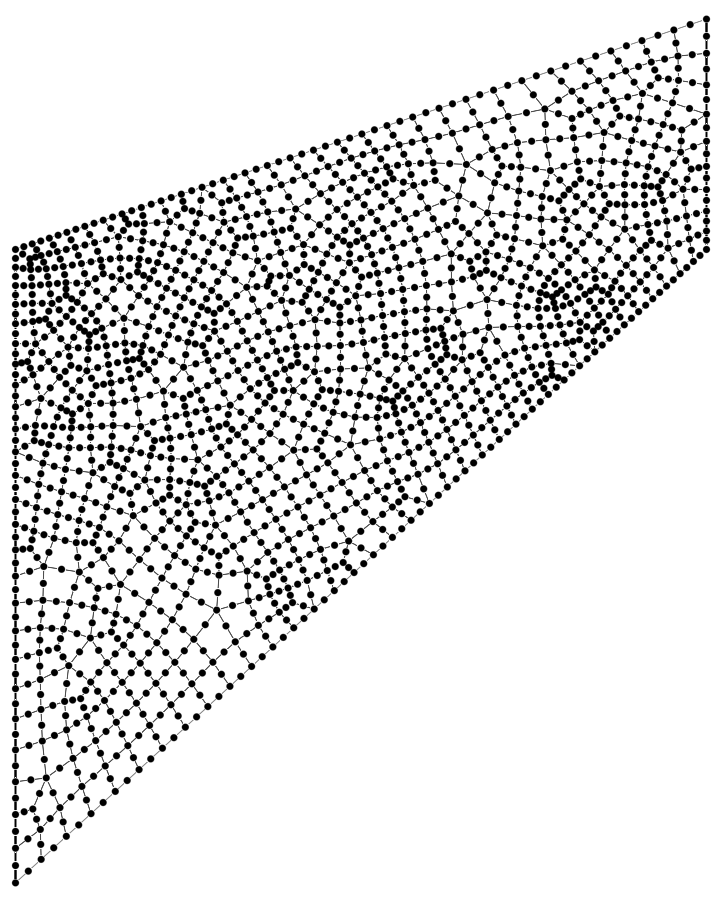
\includegraphics[width=0.33\textwidth]{png/cook_quad8_1889_msh.png}
& 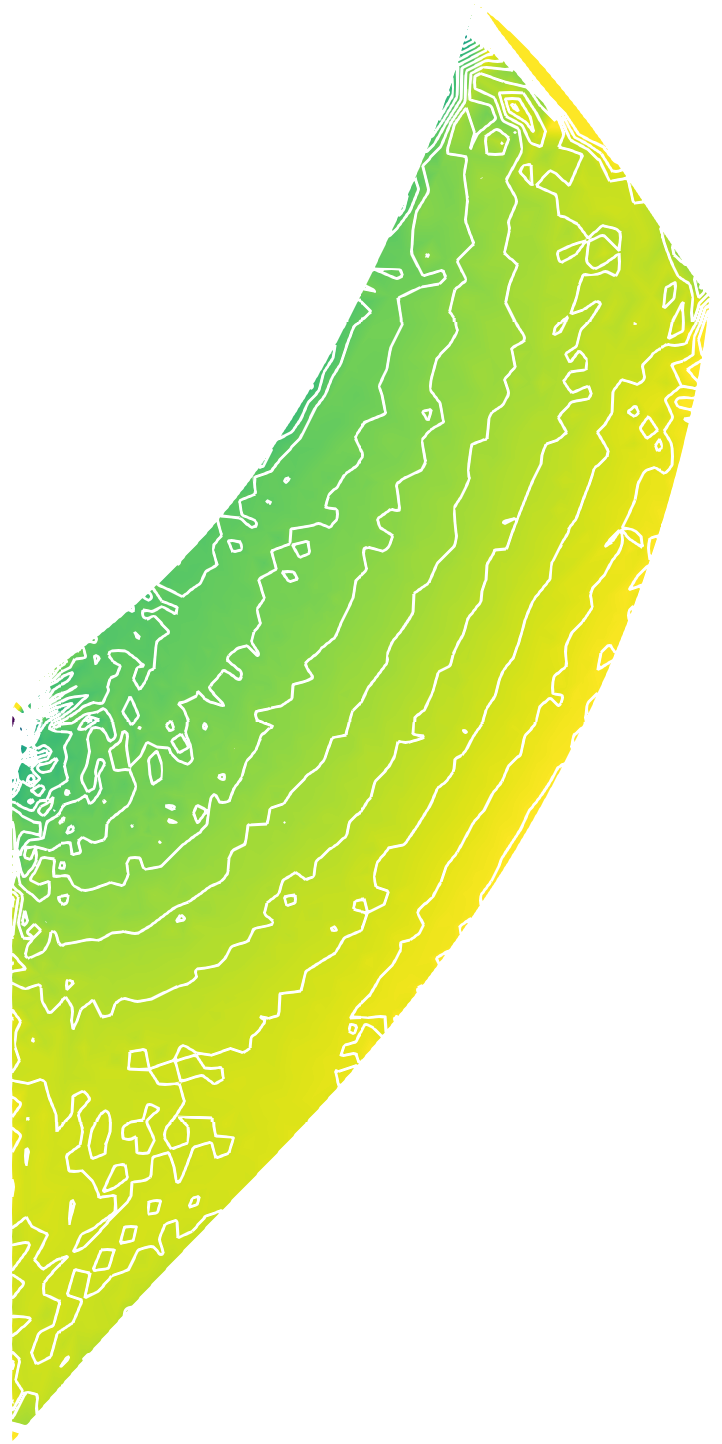
\includegraphics[width=0.28\textwidth]{png/cook_quad8_1889_1889.png}
& 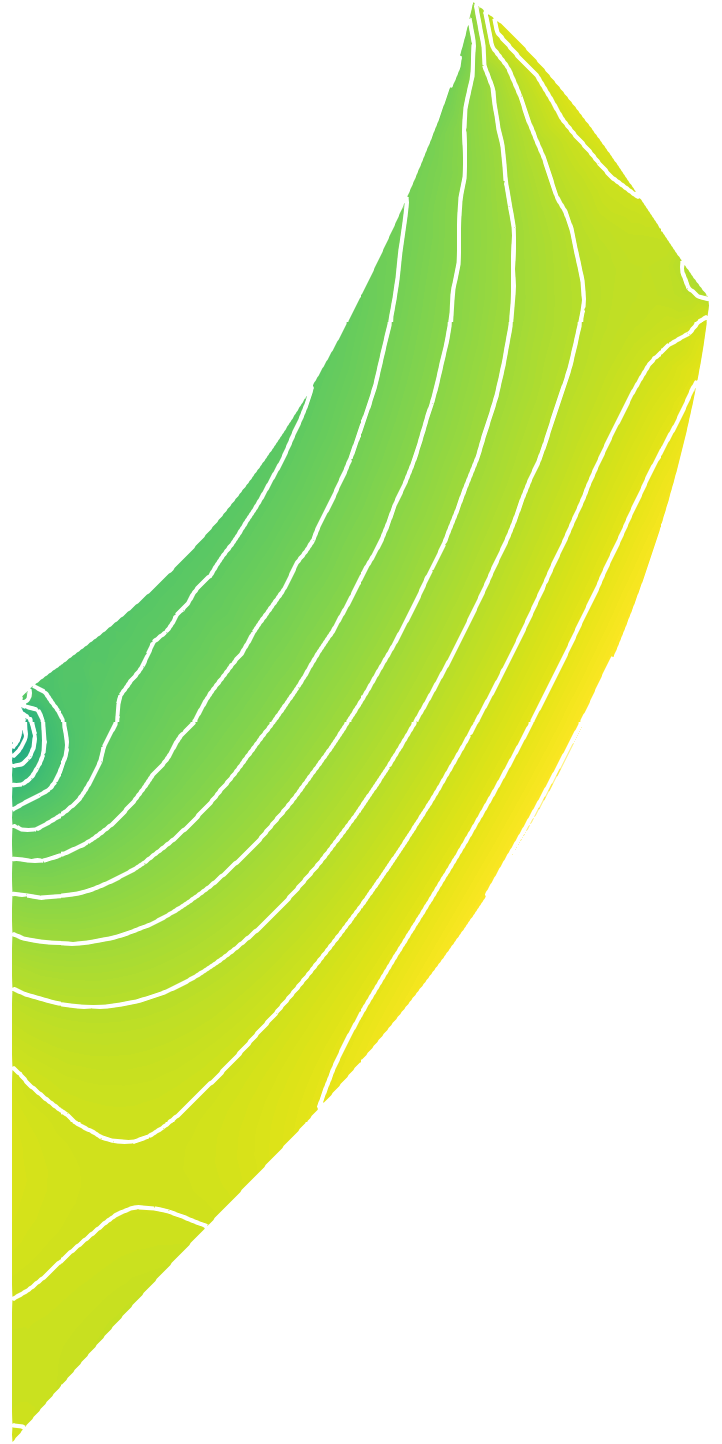
\includegraphics[width=0.28\textwidth]{png/cook_quad8_1889_647.png}
& 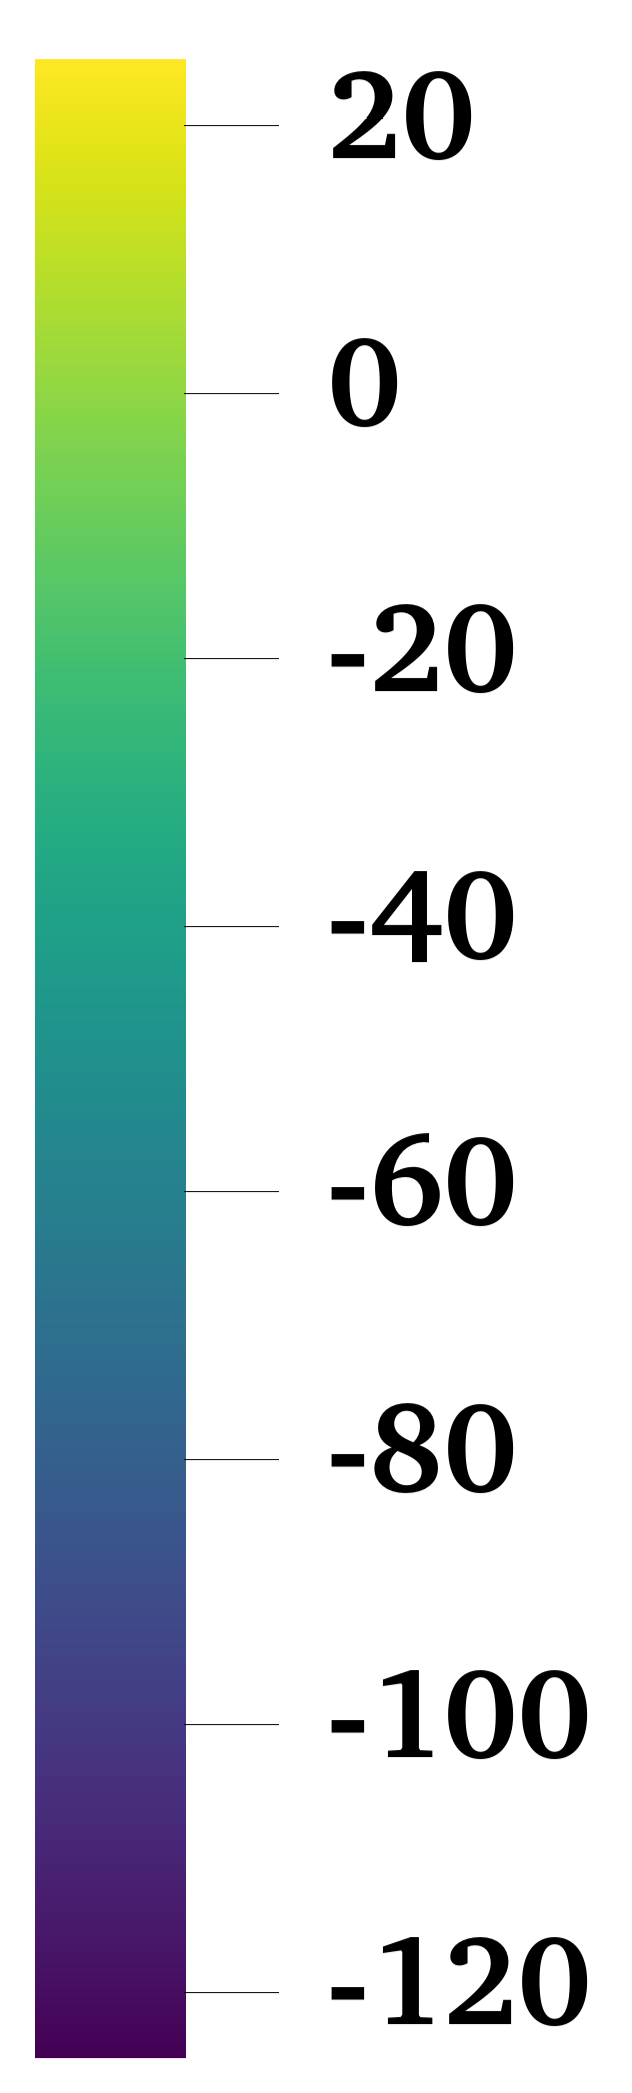
\includegraphics[width=0.1\textwidth]{png/legend.png} \\
$n_u = 1889$ & $r = n_d$ & $r = r_{opt}$ &
\end{tabular}
\caption{Comparison of pressure contour plots for Cook's membrane problem using Quad8--RK}\label{fg:cook_membrane_contour_quad8}
\end{figure}

\DIFaddbegin \DIFadd{An efficiency comparison of different methods for the Cook's membrane problem is presented in Table \ref{tab_condition}.
This includes the condition number of the global stiffness matrix and the CPU time for shape function construction, system assembly, and system solving.
The mixed FE--Meshfree formulations exhibit higher condition number and spend more time compared to the traditional element--based formulations.
This is mainly due to the implicit, complicated expression of meshfree shape functions and the larger bandwidth of the stiffness matrix, which results from the larger support size of the meshfree shape functions.
}

\begin{table}[!htp]
\centering
\caption{\DIFaddFL{Condition number and efficiency comparison for Cook's membrane problem}}
\label{tab_condition}
\begin{tabular}{ccccc}
\toprule
\multirow{2}{*}{Method} & \multirow{2}{*}{Condition number} & \multicolumn{3}{c}{\DIFaddFL{CPU--time (s) for}} \\
\DIFaddFL{\shortstack{} }& \DIFaddFL{\shortstack{} }& \DIFaddFL{Shape function }& \DIFaddFL{Assembly }& \DIFaddFL{Solving }\\
\midrule
\DIFaddFL{MINI }& \DIFaddFL{1.11E06 }& \DIFaddFL{0.025 }& \DIFaddFL{0.327 }& \DIFaddFL{0.022 }\\
\DIFaddFL{Tri3--RK($r=n_d$) }& \DIFaddFL{1.89E10 }& \DIFaddFL{1.730 }& \DIFaddFL{4.160 }& \DIFaddFL{0.108 }\\
\DIFaddFL{Tri3--RK($r=r_{opt}$) }& \DIFaddFL{1.13E08 }& \DIFaddFL{1.290 }& \DIFaddFL{1.720 }& \DIFaddFL{0.052 }\\
\DIFaddFL{T6C3 }& \DIFaddFL{1.62E05 }& \DIFaddFL{0.004 }& \DIFaddFL{0.380 }& \DIFaddFL{0.021 }\\
\DIFaddFL{Tri6--RK($r=n_d$) }& \DIFaddFL{2.48E16 }& \DIFaddFL{1.620 }& \DIFaddFL{1.670 }& \DIFaddFL{0.294 }\\
\DIFaddFL{Tri6--RK($r=r_{opt}$) }& \DIFaddFL{3.69E10 }& \DIFaddFL{1.110 }& \DIFaddFL{0.634 }& \DIFaddFL{0.077 }\\
\DIFaddFL{Q4P1 }& \DIFaddFL{5.75E12 }& \DIFaddFL{0.011 }& \DIFaddFL{0.344 }& \DIFaddFL{0.021 }\\
\DIFaddFL{Quad4--RK($r=n_d$) }& \DIFaddFL{5.21E10 }& \DIFaddFL{2.100 }& \DIFaddFL{4.890 }& \DIFaddFL{0.122 }\\
\DIFaddFL{Quad4--RK($r=r_{opt}$) }& \DIFaddFL{1.97E08 }& \DIFaddFL{1.500 }& \DIFaddFL{2.140 }& \DIFaddFL{0.057 }\\
\DIFaddFL{Q8P3 }& \DIFaddFL{2.69E07 }& \DIFaddFL{0.005 }& \DIFaddFL{0.373 }& \DIFaddFL{0.015 }\\
\DIFaddFL{Quad8--RK($r=n_d$) }& \DIFaddFL{2.75E15 }& \DIFaddFL{1.170 }& \DIFaddFL{1.180 }& \DIFaddFL{0.184 }\\
\DIFaddFL{Quad8--RK($r=r_{opt}$) }& \DIFaddFL{8.67E10 }& \DIFaddFL{0.847 }& \DIFaddFL{0.471 }& \DIFaddFL{0.065 }\\
\bottomrule
\end{tabular}
\end{table}
\DIFaddend